% This is the code that generates the slides we'll use for this section.
% If you'd simply like to view the slides, please open slides.pdf


\documentclass[10pt, aspectratio=169]{beamer}

\makeatletter
  \def\beamer@calltheme#1#2#3{%
    \def\beamer@themelist{#2}
    \@for\beamer@themename:=\beamer@themelist\do
    {\usepackage[{#1}]{\beamer@themelocation/#3\beamer@themename}}}

  \def\usefolder#1{
    \def\beamer@themelocation{#1}
  }
  \def\beamer@themelocation{}

\usefolder{../__resources__/beamer_theme}
\usetheme{nathan}

\addtobeamertemplate{navigation symbols}{}{%
    \usebeamerfont{footline}%
    \usebeamercolor[fg]{footline}%
    \hfill%
    \insertframenumber/\inserttotalframenumber
}

\title{Computational Decision Making for Regular People}
\subtitle{04: Modeling Techniques}
\date{November 5, 2024}

\usepackage[font=tiny,labelfont=bf]{caption}
\usepackage{caption}
\captionsetup[figure]{labelformat=empty}

\usepackage{listings}
\usepackage{dirtree}
\usepackage{csquotes}

\newcommand{\retirementProblem}{\textit{EXAMPLE: I have 3 retirement accounts: a Roth IRA, a 401k, and a standard brokerage account. For now, we'll assume we know the eact early return for each of these accounts: 7\%, 10\%, and 12\%. The balance on these accounts today are \$300,000, \$900,00, and \$50,000. I'm planning for 25 years of retirement. For now, we'll also assume that we'll withdraw \$8,000 per month across all the accounts (increasing 2\% per year for inflation). There are certain tax penalties for withdrawing from each account. These penalties can be complex, so for now we'll just assume that for every \$1 we withdraw, we only get \$1 $\times \alpha_a$ for withdrawing from account $a$. $\alpha_a$ values are given below. Let's assume that we make withdrawals every month. \textbf{How much should I withdraw from each account each month?}}}

\begin{document}

\begin{frame}
    \maketitle
\end{frame}

\begin{frame}{Today's Outline}
    \begin{columns}
        \begin{column}{0.5\textwidth}
            \begin{enumerate}
                \item Modeling Relationships Between Variables
                \begin{itemize}
                    \item Assignment
                    \item Knapsack 
                    \item Binary Activation
                    \item "If"
                    \item "Max" / "Min"
                \end{itemize}
                \item Modeling Real-Life Behaviors
                \begin{itemize}
                    \item Handling Multiple Sets At Once
                    \item Handling Multiple Time Periods
                    \item Handling Uncertainty
                \end{itemize}
            \end{enumerate}
            {\footnotesize \textbf{DISCLAIMER: This is not financial advice. These slides are for educational use only.}}
        \end{column}
        \begin{column}{0.5\textwidth}
            \begin{figure}
                \begin{figure}
                    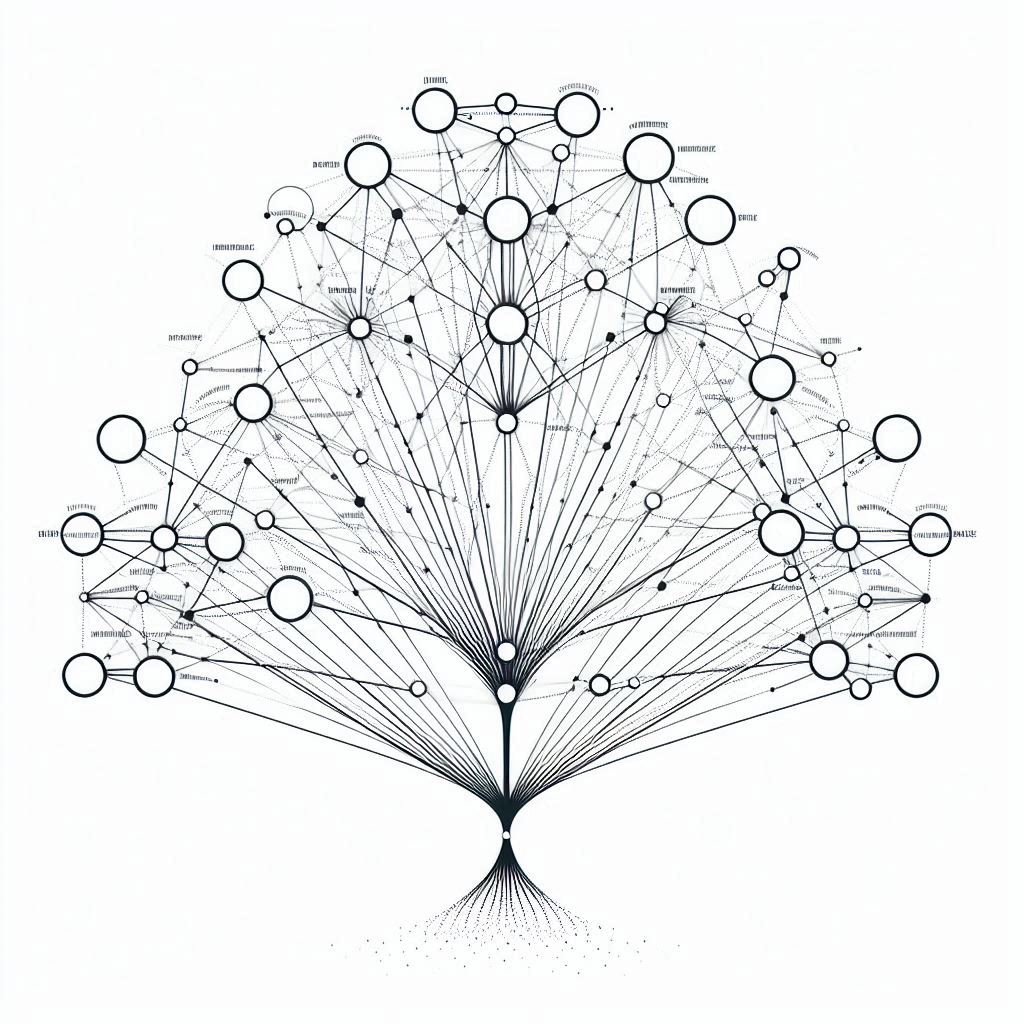
\includegraphics[width=0.95\linewidth]{DecisionTree.png}
                    \caption{This image was created with the assistance of DALL·E 3}
                \end{figure}
            \end{figure}
        \end{column}
    \end{columns}
\end{frame}

\begin{frame}{A Note on Today's Class}
    \begin{center}
        Today we're going to cover a lot of material to set us up for next week when we have to tools to address real-life problems.

        \vspace{1cm}

        We'll cover a variety of individual \enquote{tools} that are somewhat disconnected from each other.

        \vspace{1cm}

        With that in mind, I don't expect you to be 100\% confident with everything we talk about today. These slides are here to serve as your guide for implementing certain relationships. Go back and reference them often.

        \vspace{1cm}

        My goal today is mostly to \textbf{just show you what's out there}. Then, when you need a certain relationship, you can simply go look at the slide to see how to implement it.
    \end{center}
\end{frame}

\begin{frame}{Relationships Between Variables}
    \begin{itemize}
        \item For the first half of today's lesson, we'll just be focusing on how to model relationships between variables.
        \item With that in mind, we won't formulate an entire problem, \textbf{just individual parts} of a problem.
        \item We'll have examples throughout for each relationship.
        \item Use these slides as a reference:
    \end{itemize}
    \begin{center}
        \textit{I have a certain relationship I want to model, how can I do it?}

        \textit{Review these slides!}
    \end{center}
\end{frame}

\begin{frame}{The Assignment (Sub-)Problem}
    \begin{center}
        \textit{EXAMPLE: I have 5 family members and 10 chores that need to be done. I want to model the relationship that each chore has to be assigned to one person.}
    \end{center}
    \begin{columns}
        \begin{column}{0.5\textwidth}
            \begin{itemize}
                \item Sets:
                \begin{itemize}
                    \item $p \in \textbf{P}$: A set of all people.
                    \item $c \in \textbf{C}$: A set of all chores.
                \end{itemize}
                \item Variables:
                \begin{itemize}
                    \item $X_{p,c}$: In indication that chore $c$ as assigned to person $p$ ($X_{p,c} = 1$) or not ($X_{p,c} = 0$). (Binary Variable)
                \end{itemize}
            \end{itemize}
        \end{column}
        \begin{column}{0.5\textwidth}
            \begin{itemize}
                \item Constraints:
                \begin{itemize}
                    \item Each chore must be assigned to exactly one person
                    $$\sum_{p \in \textbf{P}} X_{p,c} = 1 \ \ \ \forall c \in \textbf{C}$$
                \end{itemize}
            \end{itemize}
        \end{column}
    \end{columns}
\end{frame}

\begin{frame}{The Assignment (Sub-)Problem}
    \begin{columns}
        \begin{column}{0.5\textwidth}
            \begin{itemize}
                \item It doesn't have to be \underline{chores} that are assigned to \underline{people}.
                \item It could be \underline{items} that are assigned to \underline{bins}.
                \item It could be \underline{students} that are assigned to \underline{groups}.
                \item It could be \underline{tasks} that are assigned to \underline{time periods}.
                \item ...
            \end{itemize}
        \end{column}
        \begin{column}{0.5\textwidth}
            \begin{center}
                \textit{For any} $\underline{\textbf{A}}$ \textit{that are assigned to} $\underline{\textbf{B}}$\textit{, insert the following into your model.}
            \end{center}
            \begin{itemize}
                \item Variable:
                \begin{itemize}
                    \item $X_{a,b}$: In indication that element $a$ as assigned to element $b$ ($X_{a,b} = 1$) or not ($X_{a,b} = 0$). (Binary Variable)
                \end{itemize}
                \item Constraint:
                \begin{itemize}
                    \item Each $a$ must be assigned to exactly one $b$
                    $$\sum_{b \in \textbf{B}} X_{a,b} = 1 \ \ \ \forall a \in \textbf{A}$$
                \end{itemize}
            \end{itemize}
        \end{column}
    \end{columns}
\end{frame}

\begin{frame}{The Knapsack (Sub-)Problem}
    \begin{center}
        \textit{EXAMPLE: I have 30 items that could potentially fit in my knapsack. Each item has a fixed size. My knapsack also has a fixed size. I want to model that I can't over-fill my knapsack.}
    \end{center}
    \begin{columns}
        \begin{column}{0.5\textwidth}
            \begin{itemize}
                \item Sets:
                \begin{itemize}
                    \item $i \in \textbf{I}$: A set of all items.
                \end{itemize}
                \item Parameters:
                \begin{itemize}
                    \item $\kappa_i$: The size of item $i$.
                    \item $\kappa^{KNAPSACK}$: The maximum size of my knapsack
                \end{itemize}
                \item Variables:
                \begin{itemize}
                    \item $X_{i}$: In indication that item $i$ is selected to fit in my knapsack ($X_i = 1$) or not ($X_i = 0$) (Binary Variable)
                \end{itemize}
            \end{itemize}
        \end{column}
        \begin{column}{0.5\textwidth}
            \begin{itemize}
                \item Constraints:
                \begin{itemize}
                    \item I can't overfill my knapsack
                    $$\sum_{i \in \textbf{I}} \kappa_i X_i \leq \kappa^{KNAPSACK}$$
                \end{itemize}
            \end{itemize}
        \end{column}
    \end{columns}
\end{frame}

\begin{frame}{The Knapsack (Sub-)Problem}
    \begin{columns}
        \begin{column}{0.5\textwidth}
            \begin{itemize}
                \item It doesn't have to be \underline{items} that are fit into a \underline{knapsack}.
                \item It could be \underline{students} that are fit into a \underline{group} (e.g. with a group size limit).
                \item It could be \underline{tasks} that are fit into a \underline{time period} (e.g. with a time limit).
                \item It could be \underline{major purchases} that fit into a \underline{bank account} (e.g. with a withdrawal limit).
                \item ...
            \end{itemize}
        \end{column}
        \begin{column}{0.5\textwidth}
            \begin{center}
                \textit{For any} $\underline{\textbf{A}}$ \textit{(with known size }$kappa_a$)\textit{ that has to fit into a grouping of known size} $\kappa^{TOTAL}$ \textit{insert the following into your model.}
            \end{center}
            \begin{itemize}
                \item Variable:
                \begin{itemize}
                    \item $X_{a}$: In indication that element $a$ is selected to fit into the grouping.
                \end{itemize}
                \item Constraint:
                \begin{itemize}
                    \item Each $a$ must be assigned to exactly one $b$
                    $$\sum_{a \in \textbf{A}} \kappa_a X_{a} \leq \kappa^{TOTAL}$$
                \end{itemize}
            \end{itemize}
        \end{column}
    \end{columns}
\end{frame}

\begin{frame}{Binary Activation}
    \begin{center}
        \textit{EXAMPLE: I'm considering investing in a variety of investment accounts. However, each one has a minimum deposit amount. How can I model that the amount deposited is greater than this minimum (if I open an account) or zero (if I don't)?}
    \end{center}
    \begin{columns}
        \begin{column}{0.5\textwidth}
            \begin{itemize}
                \item Parameters:
                \begin{itemize}
                    \item $\kappa^{MIN}_a$: The minimum deposit amount for account $a$
                \end{itemize}
                \item Variables:
                \begin{itemize}
                    \item $X_a$: A binary variable indicating whether or not I open account $a$
                    \item $D_a$: The amount I deposit into account $a$
                \end{itemize}
            \end{itemize}
        \end{column}
        \begin{column}{0.5\textwidth}
            \begin{itemize}
                \item Constraints:
                \begin{itemize}
                    \item Minimum Deposit Constraint
                    $$D_a \geq \kappa^{MIN}_a - \$1,000,000,000 (1-X_a)$$
                \end{itemize}
                \item It doesn't have to be $\$1,000,000,000$. It just has to be some large number.
                \item We normally call this very large number a \enquote{Big M}.
            \end{itemize}
        \end{column}
    \end{columns}
\end{frame}

\begin{frame}{\enquote{Big M} Constraints}
    \vspace{-0.4cm}
    \begin{columns}
        \begin{column}{0.5\textwidth}
            \begin{itemize}
                \item Use a Big M constraint whenever you have a upper or lower \textbf{limit that is contingent on a binary decision}.
                \item Main Idea: Include an extra term in any constraints that you want to de-activate when a binary variable is 1 (or 0). This extra term should make the constraint so loose that it'll never be binding.
                \item In general, you should just add a binary variable times some \underbar{large} parameter $\mathcal{M}$
                \item Example:
            \end{itemize}
            $$D_a \geq \kappa^{MIN}_a - \mathcal{M} (1-X_a)$$
        \end{column}
        \begin{column}{0.5\textwidth}
            \begin{figure}
                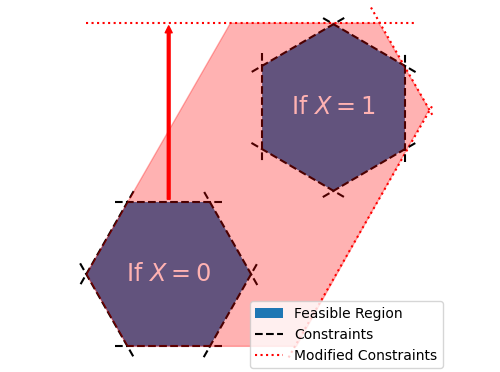
\includegraphics[width=0.8\linewidth]{ExpandedBigM.png}
            \end{figure}
        \end{column}
    \end{columns}
    \begin{itemize}
        \item NOTE OF CAUTION: Choosing a good $\mathcal{M}$ value is the name of the game here:
        \begin{itemize}
            \item Too small: You'll be chopping off parts of the true feasible region. Your problem is likely to become infeasible.
            \item Too big: The solver can get lost and can slow way down.
            \item Too too big: Your computer can't handle huge numbers and (comparatively) tiny numbers at the same time. You're likely to encounter weird errors.
        \end{itemize}
    \end{itemize}
\end{frame}

\begin{frame}{\enquote{If} Statements}
    \textit{Think of this as a generalization of a Big M constraint.}
    \begin{columns}[t]
        \begin{column}[t]{0.5\textwidth}
            \begin{itemize}
                \item Normal "if" statements look like this:
                $$A = \begin{cases}B & if\ X\\C & else \end{cases}$$
                \item We can reformulate this like this:
                $$A = A^B + A^C$$
                $$A^B = \begin{cases}B & if\ X\\0 & else \end{cases} = BX$$
                $$A^C = \begin{cases}C & if\ (1-X)\\0 & else \end{cases} = C(1-X)$$
            \end{itemize}
        \end{column}
        \begin{column}[t]{0.5\textwidth}
            \begin{itemize}
                \item As an aside, the solver will solve faster if we apply some logical tricks:
                \item We can reformulate $A = BX$ using a series of Big M Constraints:
                $$A \leq \beta^{MAX} X$$
                $$A \leq B + \beta^{MIN}(X-1)$$
                $$A \geq \beta^{MIN}X$$
                $$A \geq B + \beta^{MAX}(X-1)$$
                \item Here, $\beta^{MAX}$ and $\beta^{MIN}$ are the maximum and minimum values that $B$ is capable of being. (Big Ms)
                \item If $C$ is not 0, repeat this process for C replacing $X$ with $1-X$.
            \end{itemize}
        \end{column}
    \end{columns}
\end{frame}

\begin{frame}{\enquote{If} Statement Math ({\small If You're Interested})}
    \begin{columns}
        \begin{column}{0.5\textwidth}
            \begin{center}
                Explanation of how to come up with the linearization of $A=BX$:
                \begin{figure}
                    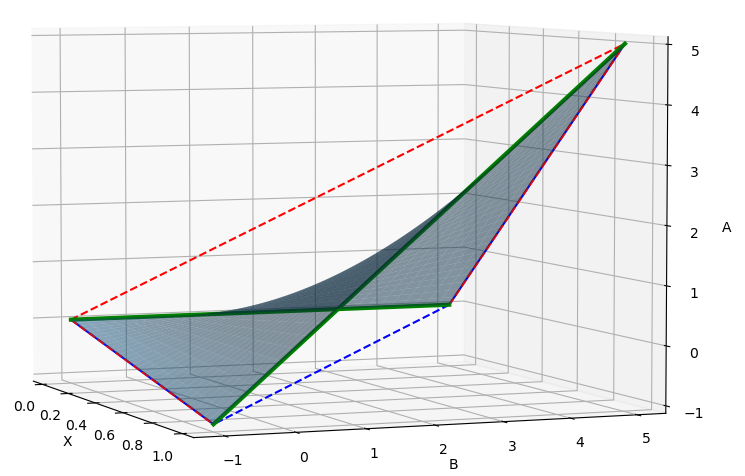
\includegraphics[width=\linewidth]{DoubleSidedBigM.png}
                \end{figure}
            \end{center}
            \begin{tabular}{c c}
                $A \leq \beta^{MAX} X$ & $A \geq \beta^{MIN}X$ \\
                $A \leq B + \beta^{MIN}(X-1)$ & $A \geq B + \beta^{MAX}(X-1)$
            \end{tabular}
        \end{column}
        \begin{column}{0.5\textwidth}

            \begin{itemize}
                \item Sometimes the objective you define indicates that $A$ will always be maximized or minimized.
                \item If you're certain that $A$ will ONLY ever be either maximized or minimized, you can drop two of the constraints.
                \begin{itemize}
                    \item Maximize $A$, drop "Greater Than" Constraints
                    \item Minimize $A$, drop "Less Than" Constraints
                \end{itemize}
                \item Dropping unnecessary constraints means there are less things for the solver to consider: The solver will go faster.
            \end{itemize}
        \end{column}
    \end{columns}
\end{frame}

\begin{frame}{If Statement Example}
    \begin{center}
        \textit{EXAMPLE: I'm buying a home. The mortgage lender offers me an interest rate of 5\%. However, for a certain upfront fee, I can buy down the interest rate to 4.5\%. How can I model the interest rate, given that it changes depending on my decision to buy down or not?}
    \end{center}
    \begin{columns}
        \begin{column}{0.5\textwidth}
            \begin{itemize}
                \item Variables:
                \begin{itemize}
                    \item $X$: An indication of whether I choose to buy down ($X=1$) or not ($X=0$).
                    \item $R$: The resulting interest rate.
                \end{itemize}
                \item Underlying Math:
                $$R = \begin{cases}
                    4.5 & X \\
                    5.0 & else
                \end{cases}$$
            \end{itemize}
        \end{column}
        \begin{column}{0.5\textwidth}
            \begin{itemize}
                \item Constraints:
                $$R^A = 4.5 X$$
                $$R^B = 5.0 (1-X)$$
                $$R = R^A + R^B$$
            \end{itemize}
        \end{column}
    \end{columns}
\end{frame}

\begin{frame}[t]{\enquote{Max} Statements}
    \begin{center}
        \textbf{IMPORTANT CONSIDERATION: Maximizing or Minimizing $A$}
    \end{center}
    \begin{columns}[t]
        \begin{column}[t]{0.5\textwidth}
            \vspace{-.8cm}
            \begin{center}
                \underbar{If you will allways be minimizing $A=max(B,C)$},
                \underbar{}
            \end{center}
            \vspace{-0.4cm}
            \begin{itemize}
                \item Model this as two individual inequalities (no binary variable needed!):
                $$A \geq B$$
                $$A \geq C$$
            \end{itemize}
            \begin{center}
                \underbar{If you'll be maximizing $A=max(B,C)$}
                \underbar{or you're not sure},
            \end{center}
            \begin{itemize}
                \item You'll need to use a binary variable with and the Big M constraints shown on the right.
            \end{itemize}
        \end{column}
        \begin{column}[t]{0.5\textwidth}
                $$B - C \leq \mathcal{M} Y$$
                $$C - B \leq \mathcal{M} (1-Y)$$
                $$A \geq B$$
                $$A \geq C$$
                $$A \leq B + \mathcal{M}(1-Y)$$
                $$A \leq C + \mathcal{M}Y$$

                Here, $\mathcal{M}$ is the maximum possible difference between $B$ and $C$ (e.g. $\max{\left|B-C\right|}$) and $Y$ is a new binary variable.
        \end{column}
    \end{columns}
\end{frame}

\begin{frame}[t]{\enquote{Min} Statements}
    \begin{center}
        \textit{Note that this is the a \enquote{Max} statement multiplied by -1.}

        \textbf{IMPORTANT CONSIDERATION: Maximizing or Minimizing $A$}
    \end{center}
    \begin{columns}[t]
        \begin{column}[t]{0.5\textwidth}
            \vspace{-.8cm}
            \begin{center}
                \underbar{If you will allways be maximizing $A=min(B,C)$},
                \underbar{}
            \end{center}
            \vspace{-0.4cm}
            \begin{itemize}
                \item Model this as two individual inequalities (no binary variable needed!):
                $$A \leq B$$
                $$A \leq C$$
            \end{itemize}
            \begin{center}
                \underbar{If you'll be minimizing $A=max(B,C)$}
                \underbar{or you're not sure},
            \end{center}
            \begin{itemize}
                \item You'll need to use a binary variable with and the Big M constraints shown on the right.
            \end{itemize}
        \end{column}
        \begin{column}[t]{0.5\textwidth}
                $$C - B \leq \mathcal{M} Y$$
                $$B - C \leq \mathcal{M} (1-Y)$$
                $$A \leq B$$
                $$A \leq C$$
                $$A \geq B - \mathcal{M}(1-Y)$$
                $$A \geq C - \mathcal{M}Y$$

                Here, $\mathcal{M}$ is the maximum possible difference between $B$ and $C$ (e.g. $\max{\left|B-C\right|}$) and $Y$ is a new binary variable.
        \end{column}
    \end{columns}
\end{frame}

\begin{frame}{Min/Max Statement Example}
    \begin{center}
        \textit{EXAMPLE: I'm buying a house. As we saw in the previous example, the interest rate for a particular lender can depend on lots of decisions. Let's say that I had two different lenders each with their own buy-down options that I model using "If" statements to prodcue $R_1$ and $R_2$. I now want to model the lesser of these two as $R^{ACTUAL}$. How can I model this?}
    \end{center}
    \begin{columns}
        \begin{column}{0.5\textwidth}
            \begin{itemize}
                \item Underlying Math:
                $$R^{ACUTAL} = \min(R_1,R_2)$$
                \item In paractice, we want low interest rates. So we'll be minimizing this minimum. So we have to use a binary variable:
            \end{itemize}
        \end{column}
        \begin{column}{0.5\textwidth}
            \begin{itemize}
                \item Constraints:
            \end{itemize}
            $$R_2 - R_1 \leq \mathcal{M} Y$$
            $$R_1 - R_2 \leq \mathcal{M} (1-Y)$$
            $$R^{ACTUAL} \leq R_1$$
            $$R^{ACTUAL} \leq R_2$$
            $$R^{ACTUAL} \geq R_1 -\mathcal{M}(1-Y)$$
            $$R^{ACTUAL} \geq R_2 - \mathcal{M} Y$$
        \end{column}
    \end{columns}
\end{frame}

\begin{frame}{Modeling Real-Life Behaviors}
    \begin{itemize}
        \item That concludes the first half of the lesson.
        \item Now we'll move on to how to model real-life problems.
        \item To do that, I'll use an example: Retirement Planning
    \end{itemize}

    \begin{center}
        \retirementProblem

        \begin{tabular}{|c|c|}
            \hline
            $a$ & $\alpha_a$ \\
            \hline \hline
            IRA & 1 \\
            \hline
            401k & 0.8 \\
            \hline
            Brokerage & 0.7 \\
            \hline
        \end{tabular}
    \end{center}
\end{frame}

\begin{frame}{Steps of Formulating a Problem}
    \begin{enumerate}
        \item Objective Function ($f(X,Y,Z,...$))
        \item Decision Variables ($X,Y,Z,...$)
        \item Parameters ($\alpha,\beta,\gamma,...$)
        \item Constraints ($X + Y \leq Z...$)
    \end{enumerate}
    \begin{itemize}
        \item Throughout: Think of relevant sets that you'd like to repeat variables and/or constraints over.
    \end{itemize}
\end{frame}

\begin{frame}{STEP 1: Identify Objective}
    \begin{columns}
        \begin{column}{0.5\textwidth}
            \retirementProblem
        \end{column}
        \begin{column}{0.5\textwidth}
            \begin{itemize}
                \item What's the objective here?
                \begin{itemize}
                    \item Hint: I didn't explicitly give it to you.
                \end{itemize}
                \pause
                \item There might be several options (depending on what you actually want).
                \item One that makes sense to me is to \textbf{maximize total ending balance}.
            \end{itemize}
        \end{column}
    \end{columns}
\end{frame}

\begin{frame}{STEP 2: Identify Variables}
    \begin{columns}
        \begin{column}{0.5\textwidth}
            \retirementProblem
        \end{column}
        \begin{column}{0.5\textwidth}
            \begin{itemize}
                \item What key variables should we consider?
                \begin{itemize}
                    \item What quantities could change based on decisions that I make?
                \end{itemize}
                \pause
                \vspace{0.5cm}
                \item $B$: The balance in a certain account.
                \item $W$: The amount I withdraw from a certain account.
                
                \pause
                \vspace{0.5cm}
                \item But what is the \enquote{balance} on a certain account?
                \begin{itemize}
                    \item Is there just one balance for all the accounts for all the months we're considering?
                    \item How can we fix this?
                \end{itemize}
            \end{itemize}
        \end{column}
    \end{columns}
\end{frame}

\begin{frame}{STEP 2a: Introduce Some Sets}
    \begin{columns}
        \begin{column}{0.5\textwidth}
            \retirementProblem
        \end{column}
        \begin{column}{0.5\textwidth}
            \begin{itemize}
                \item Sets:
                \begin{itemize}
                    \item $\textbf{A}$: A set of all accounts
                    \item $\textbf{T}$: A set of all time periods (e.g. months)
                \end{itemize}
                $$\downarrow$$
                \item $B_{a,t}$: The balance on account $a$ at the beggining of month $t$
                \item $W_{a,t}$: The amount I withdraw from account $a$ during month $t$
            \end{itemize}
        \end{column}
    \end{columns}
\end{frame}

\begin{frame}{STEP 3: Idenfity Parameters}
    \begin{columns}
        \begin{column}{0.5\textwidth}
            \retirementProblem
        \end{column}
        \begin{column}{0.5\textwidth}
            \begin{itemize}
                \item What parameters (i.e. constant values) do you see?
                \pause
                \item $\beta_a$: The initial balance on account $a$.
                \begin{itemize}
                    \item I like $\beta$ since it looks like $B$ which is the variable most related to this parameter.
                \end{itemize}
                \item $\delta_a$: The (monthly?) interest rate for account $a$.
                \item $\omega_t$: The amount of money I'll need to withdraw in month $t$
                \begin{itemize}
                    \item Remember, this depends on the month ($t$) since it changes with inflation.
                \end{itemize}
                \item $\alpha_a$: The fraction of money withdrawn from account $a$ that I get to keep.
            \end{itemize}
        \end{column}
    \end{columns}
\end{frame}

\begin{frame}{STEP 3a: Compute Parameters}
    \begin{columns}
        \begin{column}{\textwidth}
            \begin{itemize}
                \item $\delta_a$: The (monthly?) interest rate for account $a$.
                \begin{itemize}
                    \item Thinking ahead, we're going to have an equation showing the difference in account balances month-to-month (since $B_{a,t}$ is defined on a monthly basis). This equation will need this value. So it should be given on a monthly basis.
                    \item I just Google \enquote{How to convert yearly interest rate to monthly}
                    $$\delta_a = \frac{\text{Yearly Interest Rate}}{12}$$
                \end{itemize}
                \item $\omega_t$: The amount of money I'll need to withdraw in month $t$
                \begin{itemize}
                    \item I just ask ChatGPT: \enquote{I have an initial quantity of money that will increase with inflation. I know the yearly inflation rate is 2\%. Please give a formula for that this quantity will be "t" months from now.}
                    $$\omega_t = \$8,000 \times (1 + \frac{0.02}{12})^t$$
                \end{itemize}
            \end{itemize}
        \end{column}
    \end{columns}
\end{frame}

\begin{frame}{STEP 4: Idenfity Constraints}
    \begin{columns}
        \begin{column}{0.5\textwidth}
            \retirementProblem
        \end{column}
        \begin{column}{0.5\textwidth}
            \begin{itemize}
                \item What constraints do you see?
                \item If I gave you the balance for account $a$ at the beginning of month $t-1$ (i.e. $B_{a,t-1}$) along with how much you withdrew in that month (i.e. $W_{a,t-1}$), could you tell the balance in that account at month $t$?
                \pause
                \vspace{-0.2cm}
                $$B_{a,t} = \left(B_{a,t-1}-W_{a,t-1}\right) \times (1 + \delta_a)$$
                \item But wait!? How should I repeat this equation? If so, how should I repeat it?
                \pause
                \vspace{-0.2cm}
                \begin{equation}
                    \begin{split}
                    B_{a,t} = \left(B_{a,t-1}-W_{a,t-1}\right) \times (1 + \delta_a) \\ \forall a \in \textbf{A}, t \in \textbf{T}
                    \end{split} \tag*{}
                \end{equation}
                \item But what about $t=0$?
                \pause
                \vspace{-0.2cm}
                \begin{equation}
                    \begin{split}
                    B_{a,t} = \left(B_{a,t-1}-W_{a,t-1}\right) \times (1 + \delta_a) \\ \forall a \in \textbf{A}, t \in \textbf{T}^{NON-INIT}
                    \end{split} \tag*{}
                \end{equation}
            \end{itemize}
        \end{column}
    \end{columns}
\end{frame}

\begin{frame}{STEP 4: Idenfity Constraints}
    \begin{columns}
        \begin{column}{0.5\textwidth}
            \retirementProblem
        \end{column}
        \begin{column}{0.5\textwidth}
            \begin{itemize}
                \item What other constraints?
                \item If my goal is to maximize $B_{a,t}$, having zero withdrawals is a good way to get there. Should we allow this?
                \pause
                \item The Gist: Withdrawals has to be equal to $\omega_t$.
                \begin{itemize}
                    \item Hint: We have two sets here $\textbf{A}$ and $\textbf{T}$. This constraint will involve both of them, but in different ways. Can you figure out how?
                \end{itemize}
                \pause
                $$\sum_{a \in \textbf{A}} \alpha_a W_{a,t} = \omega_t \ \ \forall t \in \textbf{T}$$
                \vspace{-0.3cm}
                \item Any consideration of $\textbf{T}$ versus $\textbf{T}^{NON-INIT}$?
                \pause
                \vspace{-0.3cm}
                \begin{itemize}
                    \item No. Special considerations for the initial (or final time period) usually only happen when our constraint involves both $t$ AND $t-1$.
                \end{itemize}
            \end{itemize}
        \end{column}
    \end{columns}
\end{frame}

\begin{frame}{STEP 4: Idenfity Constraints}
    \begin{columns}
        \begin{column}{0.5\textwidth}
            \retirementProblem
        \end{column}
        \begin{column}{0.5\textwidth}
            \begin{itemize}
                \item What other constraints?
                \item Another way to get really large ending balances would be to start with infinitely large initial balances. Is this allowed?
                \pause
                \item The Gist: The initial balance should be equal to $\beta_a$.
                \item Should we repeat over $\textbf{T}$?
                \pause
                \vspace{-0.3cm}
                $$B_{a,0} = \beta{a} \ \ \forall a \in \textbf{A}$$
                \item Finally, another way to get really big ending balances would be to have negative withdrawals. Is this allowed?
                \pause
                \vspace{-0.3cm}
                $$W_{a,t} \geq 0 \ \ \forall a \in \textbf{A}, t \in \textbf{T}$$
                \item We can define this in Pyomo buy simply saying that $W_{a,t}$ is in the "NonNegativeReals" domain.
            \end{itemize}
        \end{column}
    \end{columns}
\end{frame}

\begin{frame}{Bringing It All Together}
    \begin{columns}
        \begin{column}{0.5\textwidth}
            \begin{itemize}
                \item Let's revisit the objective since we defined it only using words earlier: // \enquote{Maximize total ending balance}.
                \item Let's define it using math:
                \pause
                $$max \sum_{a \in \textbf{A}} B_{a,t^{END}}$$
                \item Now let's go gather everything from the previous slides.
                \pause
            \end{itemize}
        \end{column}
        \begin{column}{0.5\textwidth}
            $$max \sum_{a \in \textbf{A}} B_{a,t^{END}}$$
            $$----\text{ subject to }----$$
            \begin{equation}
                \begin{split}
                B_{a,t} = \left(B_{a,t-1}-W_{a,t-1}\right) \times (1 + \delta_a) \\ \forall a \in \textbf{A}, t \in \textbf{T}^{NON-INIT}
                \end{split} \tag*{}
            \end{equation}
            $$\sum_{a \in \textbf{A}} \alpha_a W_{a,t} = \omega_t \ \ \forall t \in \textbf{T}$$
            $$B_{a,0} = \beta{a} \ \ \forall a \in \textbf{A}$$
            $$W_{a,t} \geq 0 \ \ \forall a \in \textbf{A}, t \in \textbf{T}$$
            \begin{center}
                \textit{This is your sticky note to have by when you code this model in Pyomo.}
            \end{center}
        \end{column}
    \end{columns}
\end{frame}

\begin{frame}{Handling Uncertainty}
    \begin{columns}
        \begin{column}{0.5\textwidth}
            \begin{itemize}
                \item This is an active field of research. If you're interested in learning more, the words to look up are "Stochastic Programming".
                \item Scenarios ($s \in \textbf{S}$)
                \begin{itemize}
                    \item An enumeration of all possible outcomes
                    \item Each path should have an associated probability $\pi_s$
                    \item All probabilities should sum to 1 (100\%)
                \end{itemize}
                \item Coming up with these is one of the hardest parts
                \begin{itemize}
                    \item Virtually impossible to enumerate \textbf{all} outcomes.
                    \item Very hard to estimate the probability of each outcome.
                \end{itemize}
            \end{itemize}
        \end{column}
        \begin{column}{0.5\textwidth}
            \begin{figure}
                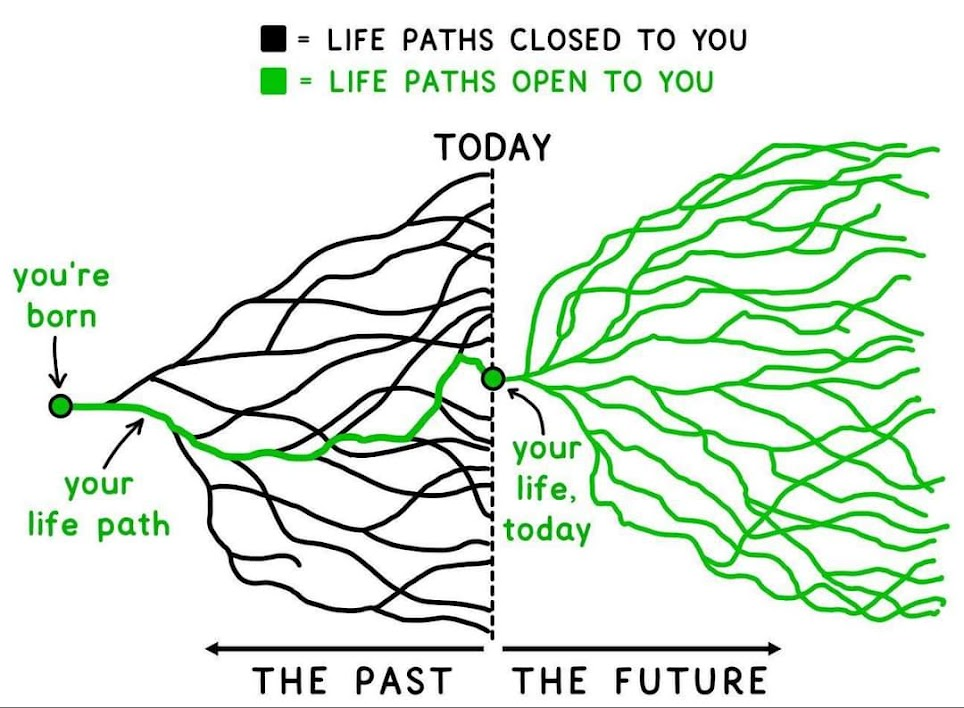
\includegraphics[width=\linewidth]{StochasticTree.jpg}
            \end{figure}
        \end{column}
    \end{columns}
\end{frame}

\begin{frame}{Handling Uncertainty (Generic)}
    \begin{columns}
        \begin{column}{0.5\textwidth}
            \begin{itemize}
                \item Some variables are shared by all scenarios
                \begin{itemize}
                    \item Decisions that need to be made here and now that impact all scenarios moving forward.
                \end{itemize}
                \item Some variables can be made in the future (and are thus specific to each scenario)
                \begin{itemize}
                    \item Each scenario get's a unique copy of that variable (e.g. iterate over \textbf{S})
                    \item But at certain points in time, certain scenarios are not yet distinguishable. In order to prevent the solution from "anticipating" future changes that are not yet clear, we need "non-anticipativity constraints"
                    \item For each box, select on representative scenario ($s_1$), all other scenarios ($s_2$) should equal that scenario 
                    \item $X_{s_1,t} = X_{s_2,t} \ \ \ \forall s_2 \in \textbf{S}^{BOX}, t \in \textbf{T}^{BOX}$
                \end{itemize}
            \end{itemize}
        \end{column}
        \begin{column}{0.5\textwidth}
            \begin{figure}
                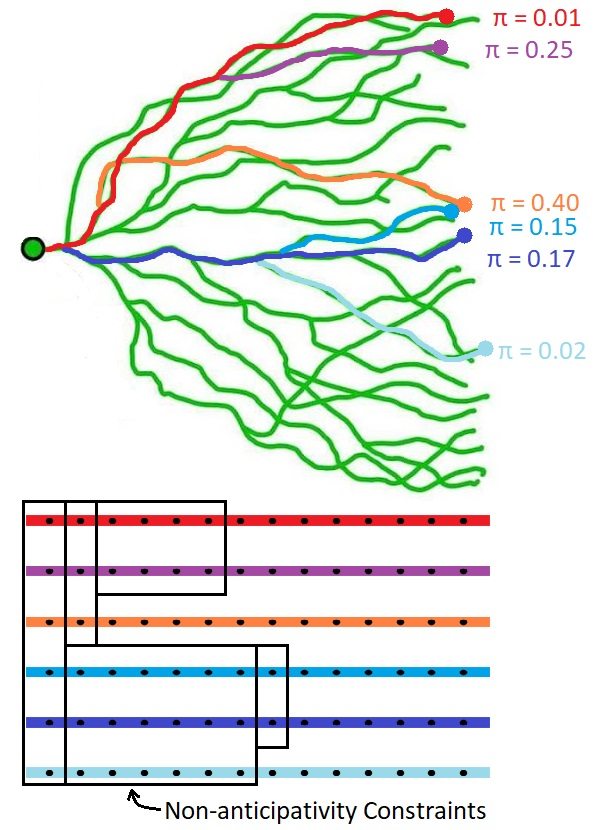
\includegraphics[width=0.75\linewidth]{StochasticTreeHighlight.jpg}
            \end{figure}
        \end{column}
    \end{columns}
\end{frame}

\begin{frame}{Handling Uncertainty (Typical)}
    \begin{itemize}
        \item A tree-like structure can be unreasonably difficult for even a computer to solve if we have a LOT of scenarios that are all interconnected.
        \item A simplification that works well is called a "two-stage" approach.
    \end{itemize}
    \begin{columns}
        \begin{column}{0.5\textwidth}
            \begin{enumerate}
                \item Assume that you make one set of choices today that will be constant regardless of which path you take. I'll call these "policy variables" (a.k.a. \enquote{$1^{st}$ stage variables}).
                \item Then assume that all scenarios are totally independent.
                \item Apply the policy decisions to each scenario.
                \begin{itemize}
                    \item Each scenario will have it's own set of unique "scenario variables" that will be determined as a result of the policy variables. (a.k.a. \enquote{$2^{nd}$ stage variables})
                \end{itemize}
            \end{enumerate}
        \end{column}
        \begin{column}{0.5\textwidth}
            \begin{figure}
                \includegraphics[width=\linewidth]{TwoStageStochastic.jpg}
            \end{figure}
        \end{column}
    \end{columns}
\end{frame}

\begin{frame}{Two-Stage Example}
    \begin{columns}
        \begin{column}{0.5\textwidth}
            \begin{itemize}
                \item Imagine I have the same retirement planning problem we had earlier.
                \item But now, instead of knowing the exact rate of return for each account at each month, we know some possible scenarios ($s$)
            \end{itemize}
            \begin{tabular}{|c|c||c|c|c|}
                \hline
                $s$ & $\pi_s$ & IRA & 401k & Brokerage \\
                \hline \hline
                1 & 0.05 & 2\% & 3\% & -2\% \\
                \hline
                2 & 0.10 & 7\% & 6\% & 20\% \\
                \hline
                3 & 0.60 & 7\% & 10\% & 12\% \\
                \hline
                4 & 0.25 & 8\% & 5\% & 0\% \\
                \hline
            \end{tabular}
        \end{column}
        \begin{column}{0.5\textwidth}
            \begin{itemize}
                \item The first thing we need to do is establish some \enquote{policy variables}.
                \begin{itemize}
                    \item My policy is that I'll withdraw a certain porportion from each account each month.
                    \item For example, perhaps I'll draw out 30\% of my monthly expenses from my IRA, 60\% from my 401k, and 10\% from my brokerage.
                    \item But I don't know the best percentage values: 30\%, 60\%, 10\%. We'll use the solver to find the optimal policy.
                \end{itemize}
                \item You can think of these policy variables repeated for all the different scenarios. But since the Non-anticipativity constraint would make them all equal, we'll only define \textbf{one set of policy variables that we'll apply to all the scenarios}.
            \end{itemize}
        \end{column}
    \end{columns}
\end{frame}

\begin{frame}{Two-Stage Example}
    \begin{columns}
        \begin{column}{0.5\textwidth}
            \begin{itemize}
                \item Policy Variables:
                \begin{itemize}
                    \item $F_a$: The fraction of my monthly expenses that I'll withdraw from account $a$
                \end{itemize}
                \item Policy Constraints:
                \begin{itemize}
                    \item Fractions must add up to 1 (i.e. 100\%)
                    $$\sum_{a \in \textbf{A}} F_a = 1$$
                \end{itemize}
                \item Now we need to modify our original problem in three ways:
                \begin{enumerate}
                    \item We need to repeat the original problem for each scenario.
                    \item We need to relate each $W$ value to our policy variables.
                    \item We need to modify the objective to account for the scenarios.
                \end{enumerate}
            \end{itemize}
        \end{column}
        \begin{column}{0.5\textwidth}
            \begin{enumerate}
                \item Repeat the original problem for each scenario.
            \end{enumerate}
            $$max \sum_{a \in \textbf{A}} B_{a,t^{END},s}$$
            $$----\text{ subject to }----$$
            \begin{equation}
                \begin{split}
                B_{a,t,s} = \left(B_{a,t-1,s}-W_{a,t-1,s}\right) \times (1 + \delta_{a,s}) \\ \forall a \in \textbf{A}, t \in \textbf{T}^{NON-INIT}, s \in \textbf{S}
                \end{split} \tag*{}
            \end{equation}
            $$\sum_{a \in \textbf{A}} \alpha_a W_{a,t,s} = \omega_t \ \ \forall t \in \textbf{T}, s \in \textbf{S}$$
            $$B_{a,0,s} = \beta{a} \ \ \forall a \in \textbf{A}, s \in \textbf{S}$$
            $$W_{a,t,s} \leq 0 \ \ \forall a \in \textbf{A}, t \in \textbf{T}, s \in \textbf{S}$$
            $$\sum_{a \in \textbf{A}} F_a = 1$$
        \end{column}
    \end{columns}
\end{frame}

\begin{frame}{Two-Stage Example}
    \begin{columns}
        \begin{column}{0.5\textwidth}
            \begin{enumerate}
                \setcounter{enumi}{1}
                \item Relate each $W$ value to our policy variables.
            \end{enumerate}
            $$max \sum_{a \in \textbf{A}} B_{a,t^{END},s}$$
            $$----\text{ subject to }----$$
            \begin{equation}
                \begin{split}
                B_{a,t,s} = \left(B_{a,t-1,s}-W_{a,t-1,s}\right) \times (1 + \delta_{a,s}) \\ \forall a \in \textbf{A}, t \in \textbf{T}^{NON-INIT}, s \in \textbf{S}
                \end{split} \tag*{}
            \end{equation}
            $$\alpha_a W_{a,t,s} = \omega_t F_a \ \ \forall a \in \textbf{A}, t \in \textbf{T}, s \in \textbf{S}, $$
            $$B_{a,0,s} = \beta{a} \ \ \forall a \in \textbf{A}, s \in \textbf{S}$$
            $$W_{a,t,s} \leq 0 \ \ \forall a \in \textbf{A}, t \in \textbf{T}, s \in \textbf{S}$$
            $$\sum_{a \in \textbf{A}} F_a = 1$$
        \end{column}
        \begin{column}{0.5\textwidth}
            \begin{enumerate}
                \setcounter{enumi}{2}
                \item Modify the objective to account for the scenarios.
            \end{enumerate}
            $$max \sum_{s \in \textbf{S}} \pi_s \sum_{a \in \textbf{A}} B_{a,t^{END},s}$$
            $$----\text{ subject to }----$$
            \begin{equation}
                \begin{split}
                B_{a,t,s} = \left(B_{a,t-1,s}-W_{a,t-1,s}\right) \times (1 + \delta_{a,s}) \\ \forall a \in \textbf{A}, t \in \textbf{T}^{NON-INIT}, s \in \textbf{S}
                \end{split} \tag*{}
            \end{equation}
            $$\alpha_a W_{a,t,s} = \omega_t F_a \ \ \forall a \in \textbf{A}, t \in \textbf{T}, s \in \textbf{S}, $$
            $$B_{a,0,s} = \beta{a} \ \ \forall a \in \textbf{A}, s \in \textbf{S}$$
            $$W_{a,t,s} \leq 0 \ \ \forall a \in \textbf{A}, t \in \textbf{T}, s \in \textbf{S}$$
            $$\sum_{a \in \textbf{A}} F_a = 1$$
        \end{column}
    \end{columns}
\end{frame}



\begin{frame}{Two-Stage Example Comments}
    \begin{itemize}
        \item I can have as many scenarios as I want (so long as my computer can handle it)
        \item The policy structure can get very nuanced. I've just proposed a very simple one here.
        \item The danger here is that the scenarios I pick have to represent reality well. (That's why Wallstreet exists)
    \end{itemize}
\end{frame}

\end{document}